\documentclass{standalone}
\usepackage{tikz}
\usetikzlibrary{calc}

\begin{document}

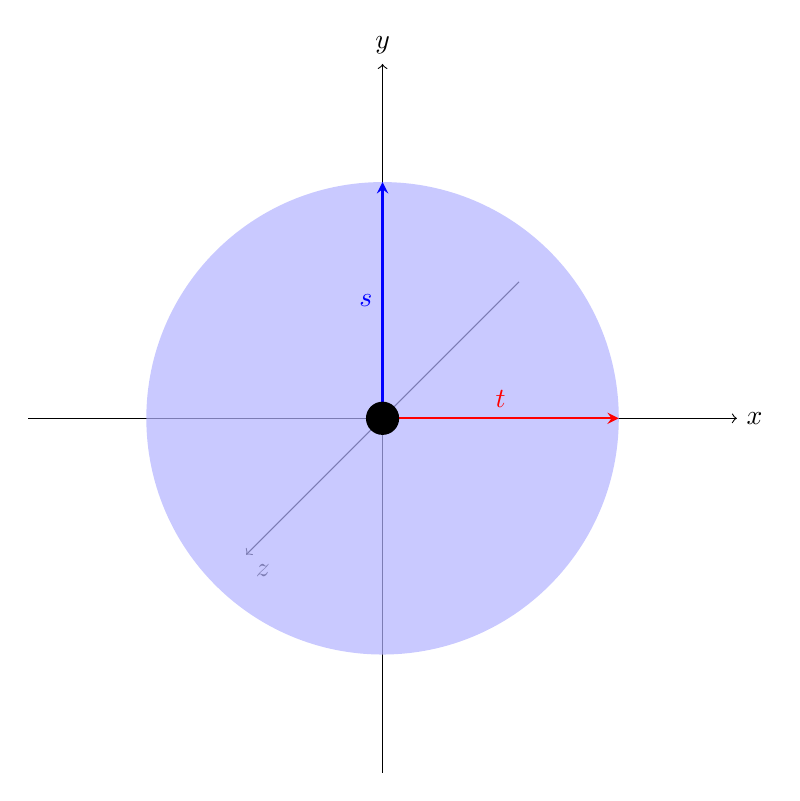
\begin{tikzpicture}[scale=3]

    % Draw the x-axis
    \draw[->] (-1.5,0,0) -- (1.5,0,0) node[right]{$x$};

    % Draw the y-axis
    \draw[->] (0,-1.5,0) -- (0,1.5,0) node[above]{$y$};

    % Draw the z-axis
    \draw[->] (0,0,-1.5) -- (0,0,1.5) node[below right]{$z$};

    % Draw the unit sphere S^2
    \fill[blue!30, opacity=0.7] (0,0,0) circle (1);

    % Draw the vector t (unit vector)
    \coordinate (O) at (0,0,0);
    \coordinate (T) at (1,0,0); % Example: t = (1, 0, 0)
    \draw[-stealth, thick, red] (O) -- (T) node[midway, above] {$t$};

    % Draw the vector s (orthogonal to t)
    \coordinate (S) at (0,1,0); % Example: s = (0, 1, 0)
    \draw[-stealth, thick, blue] (O) -- (S) node[midway, left] {$s$};

    % Draw a small dot to indicate the origin
    \fill (0,0,0) circle (2pt);

\end{tikzpicture}

\end{document}